\chapter{Исследовательская часть}

В этой части представляются технические характеристики устройства,
проведение исследования быстродействия программы и его результаты.

\section{Технические характеристики}

Спецификации устройства, использованного для тестирования:
\begin{itemize}[label=--]
	\item оперативная память 16 ГБ;
	\item процессор Intel(R) Core(TM) i7-9750H с тактовой частотой 2.60 ГГц;
	\item 6 физических и 12 логических ядер;
	\item операционная система Windows 10 Домашняя 64-разрядная с версией 22H2.
\end{itemize}

Устройство было нагружено только встроенными приложениями и подключено в сеть электропитания. 

\section{Проведение исследований}

Целью исследований является определение зависимостей: 
\begin{itemize}[label=--]
	\item времени визуализации сцены от количества полигонов;
	\item времени визуализации сцены от количества генерируемых примитивов;
	\item времени визуализации сцены от геометрических параметров примитива.
\end{itemize}

По результатам исследований должны быть составлены таблицы и построены графики зависимости.

\subsection{Исследование зависимости времени визуализации от количества полигонов}

Исследование проводится с использованием многогранника, где каждая грань соответствует отдельному полигону. Для визуализации сцены выбран <<теневой>> режим, так как он является наиболее ресурсоемким из доступных в программе.

Для каждого многогранника время визуализации измеряется трижды, после чего вычисляется среднее значение. Все замеры производятся в секундах.

Результаты определения зависимости времени визуализации сцены от количества полигонов приведены в таблице~\ref{tbl:research1}.

\begin{table}[h]
	\small
	\centering
	\caption{Зависимость времени визуализации сцены от количества полигонов}
	\begin{tabular}{|c|c|}
		\hline
		\textbf{Количество полигонов, шт.} & \textbf{Время визуализации, сек.} \\
		\hline
		10  & 5.01 \\
		20  & 7.40 \\
		30  & 8.37 \\
		40  & 8.73 \\
		50  & 9.13 \\
		60  & 9.55 \\
		70  & 10.00 \\
		80  & 10.38 \\
		90  & 10.85 \\
		100 & 11.29 \\
		\hline
	\end{tabular}
	\label{tbl:research1}
\end{table}

По таблице~\ref{tbl:research1} был построен график~\ref{fig:research1}, который наглядно демонстрирует результаты определения зависимости времени визуализации сцены от количества полигонов. Исходя из графика можно сделать вывод, что данная зависимость близка к линейной.

\begin{figure}[h] 
	\centering
	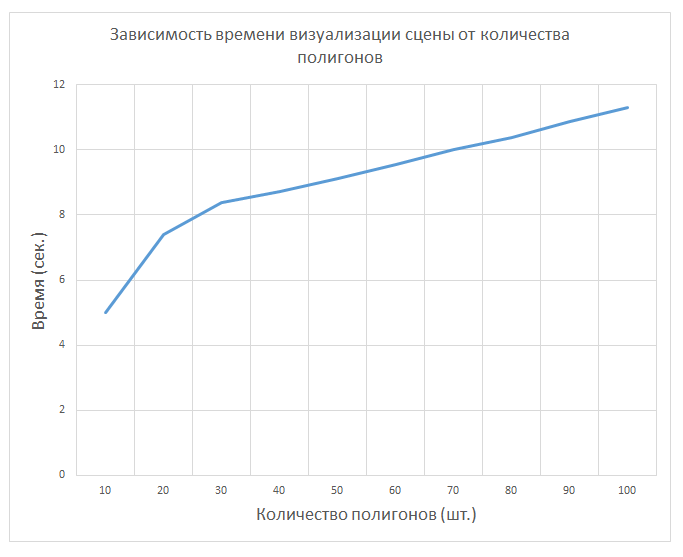
\includegraphics[width=0.97\textwidth]{images/research1.png}
	\caption{Зависимость времени визуализации сцены от количества полигонов} 
	\label{fig:research1} 
\end{figure}

\subsection{Исследование зависимости времени визуализации от количества генерируемых примитивов}

Исследование проводится с использованием многогранников, имеющих 5, 8 и 11 полигонов. Для визуализации сцены выбран <<теневой>> режим, так как он является наиболее ресурсоемким из доступных в программе.

Для каждой сцены время визуализации измеряется трижды, после чего вычисляется среднее значение. Все замеры производятся в секундах.

Результаты определения зависимости времени визуализации сцены от количества примитивов приведены в таблице~\ref{tbl:research2}.

\begin{table}[ht]
	\small
	\begin{center}
		\begin{threeparttable}
			\caption{Зависимость времени визуализации сцены от количества генерируемых примитивов}
			\begin{tabular}{|c|c|c|c|}
				\hline
				& \multicolumn{3}{c|}{\bfseries Время визуализации, сек.} \\ \cline{2-4}
				\bfseries Количество многогранников, шт. & \bfseries 5 полигонов & \bfseries 8 полигонов & \bfseries 11 полигонов \\
				\hline
				10  & 79.26   & 133.73 & 155.58  \\
				20  & 143.39 & 238.64 & 283.68  \\
				30  & 220.86 & 367.91 & 437.72  \\
				40  & 298.33 & 497.18 & 591.75  \\
				50  & 375.81 & 626.45 & 745.79  \\
				60  & 453.28 & 755.72 & 899.82  \\
				70  & 530.76 & 884.99 & 1053.86 \\
				80  & 608.23 & 1014.26 & 1207.89 \\
				90  & 685.70 & 1143.53 & 1361.93 \\
				100 & 763.18 & 1272.80 & 1515.96 \\
				\hline
			\end{tabular}	
			\label{tbl:research2}
		\end{threeparttable}
	\end{center}
\end{table}

По таблице~\ref{tbl:research2} был построен график~\ref{fig:research2}, который наглядно демонстрирует результаты определения зависимости времени визуализации сцены от количества генерируемых примитивов. Исходя из графика можно сделать вывод, что данная зависимость близка к линейной.

\clearpage

\begin{figure}[h] 
	\centering
	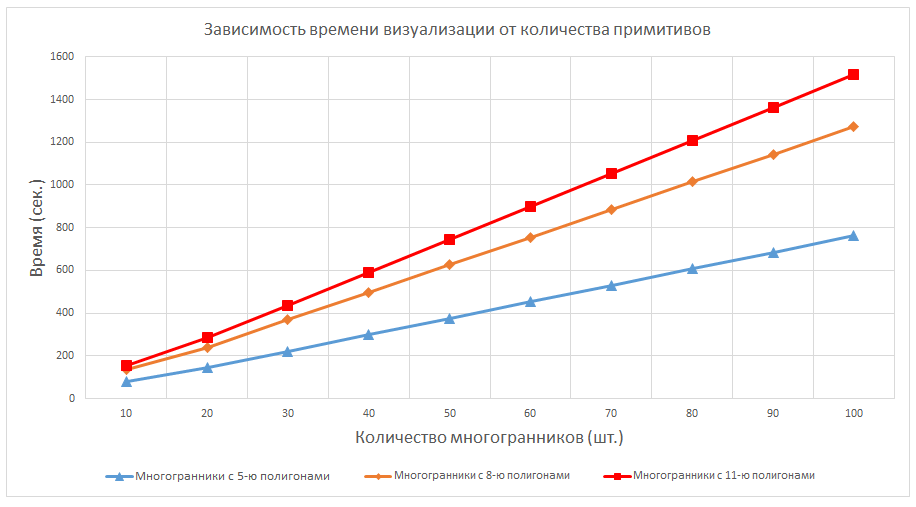
\includegraphics[width=1\textwidth]{images/research2.png}
	\caption{Зависимость времени визуализации сцены от количества примитивов} 
	\label{fig:research2} 
\end{figure}

\subsection{Исследование зависимости времени визуализации от геометрических параметров примитива}

Исследование проводится с использованием куба, так как программа позволяет изменять длину его ребра. Для визуализации сцены выбран <<теневой>> режим, так как он является наиболее ресурсоемким из доступных в программе.

Для каждого куба время визуализации измеряется трижды, после чего вычисляется среднее значение. Все замеры производятся в секундах.

Результаты определения зависимости времени визуализации сцены от количества примитивов приведены в таблице~\ref{tbl:research3}

По таблице~\ref{tbl:research3} был построен график~\ref{fig:research3}, который наглядно демонстрирует результаты определения зависимости времени визуализации сцены от размера примитива. Исходя из графика можно сделать вывод, что данная зависимость имеет явный нелинейный характер.

\clearpage

\begin{table}[h]
	\small
	\centering
	\caption{Зависимость времени визуализации сцены от размера примитива}
	\begin{tabular}{|c|c|}
		\hline
		\textbf{Длина ребра куба, у. е.} & \textbf{Время визуализации, сек.} \\
		\hline
		100  & 9.23 \\
		200  & 31.08 \\
		300  & 79.52 \\
		400  & 154.57 \\
		500  & 256.21 \\
		600  & 384.42 \\
		700  & 539.30 \\
		800  & 720.73 \\
		900  & 928.79 \\
		1000 & 1163.44 \\
		\hline
	\end{tabular}
	\label{tbl:research3}
\end{table}

\begin{figure}[h] 
	\centering
	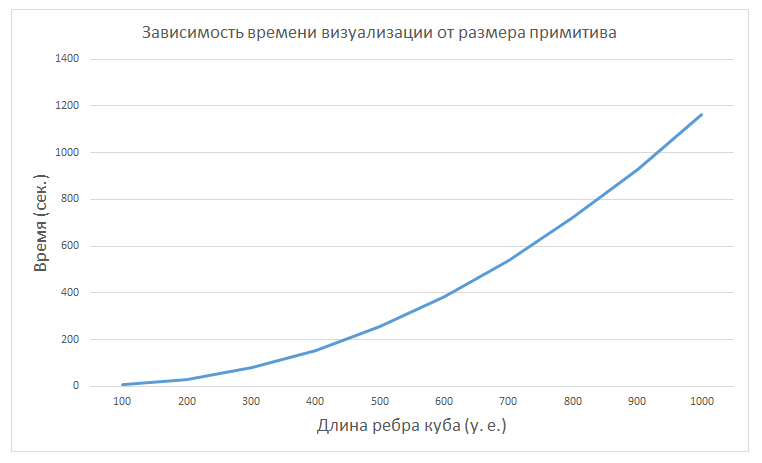
\includegraphics[width=1\textwidth]{images/research3.png}
	\caption{Зависимость времени визуализации сцены от размера примитива} 
	\label{fig:research3} 
\end{figure}

\section{Вывод}

В этой части были представлены технические характеристики устройства,
проведено исследование быстродействия программы и приведены его результаты.

\clearpage
